\chapter{if conversion \Author{C. Bruel}}
\numberofpages{10}
\graphicspath{{img/}{/if_conversion/img}{part4/if_conversion/img/}}

\newcommand\cond{~?~}

\section{Overview/Motivations}

If-conversion is the process to remove conditional branches, merging different control paths, allocating predicates to the instructions and merging the basic blocks together to generate an equivalent basic block composed of conditional instructions.
Removing branches is beneficial for several reason. it increase Instruction Level Parallelism by enlarging the size of the basic blocks, it increases cache locality and remove long latencies branches. However this is a complex task for a compiler. either done locally using peepholes or intrinsics, or scoping larger regions such hyperblocks, moving multiple control paths together can easely exceed processors resources (leading to exesive register pressure) or move unfrequently used expensive instruction (memory loads) into the critical path. 
This transforms control flow dependencies into data flow dependencies.
Thanks to partially or fully predicated Instruction Set Architecture. 
This optimisation needs a very strong knowledge of the target machine to decide how (predication, speculation, conditional moves, predicate computation and merge)to decide how complex control flow region (an hyperblock) can be transformed into an equivalent set of conditionalized instruction. So it is usually limited to compiler backends and are target specifics.

As an optimisation, the region to if-conversion must be large enough to enlarge the scope of scheduling framework, but in the same time it must not exceed the machine resources (registers, cpus). We must make sure that the newly formed basic block doesn't have a higher schedule estimation than the one that would have been taken if the code was not if-converted. If-conversion removes instructions, but also can add some overhead (new instructions to merge predicates, register pressure for speculative conditional, bigger dependence height for predicated conditionals). This framework allows the decision functions to be accurate enough to avoid beeing too conservative and aggresively if-convert code. 
\subsection{Architectural requirements}
We suppose that the target architectures has a way to emit conditional execution of instruction. This is usually achieved in 3 different ways: In this chapter we use following notation for the simple $x = p \cond a + b : 0$ assignment.

\begin{figure}
\begin{minipage}[t]{4cm}
\mbox{fully predicated:} \\
$ p \cond x = a + b $ \\
$ \overline{p} \cond x = 0 $ \\
\end{minipage}
\begin{minipage}[t]{4cm}
\mbox{partially predicated:} \\
$t = a + b $ \\
$p \cond x = t $ \\
$\overline{p} \cond x = 0 $ \\
\end{minipage}
\begin{minipage}[t]{4cm}
\mbox{$select$ instruction:} \\
$t = a + b $ \\
$x = select \; p \cond t : 0 $ \\
\end{minipage}
\end{figure}

During this SSA algorithm, we view the if-conversion into 2 different problems. First as a global problem the region to if-convert must be defined, using objective functions and branch probabilities to avoid moving to the hot path less frequently used instruction. Since if-conversion also transforms control flow dependencies into data flow dependencies, register pressure can dependencies can become significantly high.
Then as a local problem, for each basic block considered into the region, a predicate must be computed and assigned to the corresponding instructions. Finally predicated or speculative instructions must be emitted into the IR.

Conventional approaches is to use a top down hyperblock frameworks (refs) to detect interesting regions, using heuristics to predicts the beneficibility and then an if-conversion algorithm for predicate assignment and reductions. This is usually poor because resources dependencies height (due to data flow dependencies introduced by new predicates) are very difficult to predict globally. Also Such regions are usually isolated from the rest of the control flow graph using tail dupication. Finally variable renaming needs to be performed an join point expressed conditionally. 
Consider a small region: SSA naturally solves 2 other the local questions for if-conversion

\begin{figure}
\begin{minipage}[t]{4cm}
$r_1 = 1 $ \\
$ if (c) $ \\
$ \{ $ \\
\hspace*{2mm} $ l = 2 $ \\
\hspace*{2mm} $ 2 = l+3 $ \\
$ \} $ \\
$ r=\phi(r_1,r_2) $ \\
$ return r $ 
\end{minipage}
\end{figure}

1) $r$ will live simultaneously after the two paths merge, without additional renaming.
2) Which register need to be conditionalized ? in other word, what is the smallest predicate set for each variable is the best connection to each definition. e.g l depends on true predicate (no conditional use) and so can be naturally speculated while r depends on the c condition and must be predicated.

SSA is fits naturally to the if-conversion framework since renaming was performing during SSA construction, variables that need a conditional have a joined in the phi. Otherwise speculated remove the need of predicate reduction.

This algorithm takes as input SSA form and produces eith PSI-SSA if predicated instructions are available or pure SSA using select instructions to realized join points.

multiple definition problem introduced by predication: In order to perform if-conversion the architecture most provide some kind of conditional selection of operands. If such operation exist, the algorithm produces SSA to SSA form.
however, with predication we introduce a renaming problem because r is only partially redefined in the second assignment, but two definition exist. In order for the algorithm to works with SSA properties we choose to materialize using psi

\section{SSA transformations}

Before describing the global framework, we define a set of SSA operations aiming at locally reducing the control flow.:
We first consider simple transformation, walking the control flow in post order.
TODO: define ``simple regions''

    \subsection{Scope}

    \subsection{SSA operations on basic blocks}

\begin{figure}
\begin{minipage}[t]{5cm}
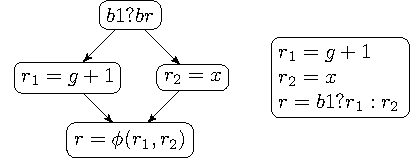
\includegraphics[scale=0.2]{phi_removal.pdf}
\caption{phi removal}
\end{minipage}
\begin{minipage}[t]{5cm}
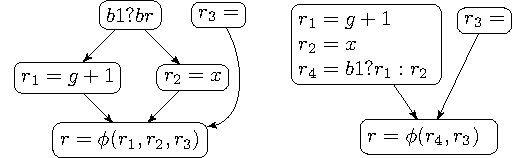
\includegraphics[scale=0.2]{phi_reduction.pdf}
\caption{phi reduction}
\end{minipage}
\begin{minipage}[t]{6cm}
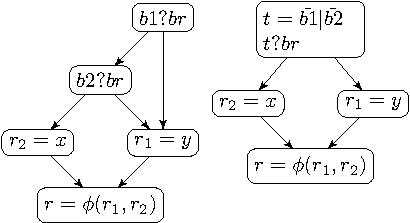
\includegraphics[scale=0.2]{phi_merge.pdf}
\caption{predicate merge}
\end{minipage}
\begin{minipage}[t]{5cm}
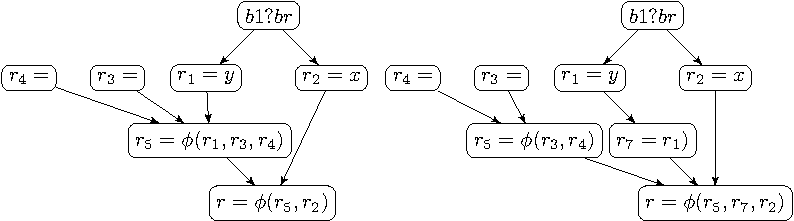
\includegraphics[scale=0.2]{phi_augmentation.pdf}
\caption{phi augmentation}
\end{minipage}
\label{fig: phi_operations}
\end{figure}

These operation are performed iterativelly on post order, consequently one of the propriety of the algorithms is that psi can be predicated. A Partial out of SSA can be iteratively performed on those regions by removing the $\phi$s and maintening a correct SSA internal representation. The algorithm takes SSA as input and produces SSA if a select instruction is available or PSI SSA if predicated instructions are available. 

    \subsection{SSA maintenance}

In this example we consider the single exit region compoled of the basic block the region be composed of the basic blocks ${H, B, C, E}$ with $H$ the head and $E$ the merging point of $B$ and $C$. 

    \subsubsection{$\phi$ removal} 
$B$ and $C$ are in the dominance frontier of $E$. After they have been merged into $H$, the new dominance frontier of $D$ becomes empty and so the $\phi$ can be removed. All the basic blocks dominated by $E$ are also dominated by $H$ (because $H$ dominated $E$ so the dominance tree is not modified)
    \subsubsection{$\phi$ reduction} 
The join block $E$ has $n$ predecessors with $n$ > 2, and $n$ blocks in its dominance frontier if it contains $\phi$s. After $B$ and $C$ removal(their content is promoted to $H$), $H$ is now in the dominance frontier of $E$, so a new $\phi$ must be created containing $n-1$ operands to maintain the SSA representation.
    \subsubsection{$\phi$ augmentation} 
The objective is to remove incoming edges into the region. if $C$ has more that 1 predecessor (one of which is $H$. $C$ is in the dominance frontier of $H$ and $E$. To remove the incoming edge, the $\phi$ must be reduced by one parameter (if it had 2 predecessors it becomes a copy). To do this we duplicate $C$ into $C'$, carrefully remaining all locals not live out outside the region. Now since $D$ has a new incoming edge (C') it's phi must be extended with the newly created duplicated definition. 
Since the algorithm works the control flow in post order mode, the dominator tree doesn't change, and it's possible to maintain the SSA locally to the inner region. By recurence the if-converted region can be in turn be optimized out if it's head belongs to the dominance frontier of an outer region.

    \subsection{$\phi$ and $\psi$ speculation properties}

Since the algorithm process the regions from inner to outer, conditional operations will be in turn speculated or reconditionalized with a new condition. We define here $\phi$ operand promotion rules.

    \subsubsection{Partial redefinition problem}

The psi exposes the control flow dependencies to the data flow, by expressing the merge of two definitions. Note that the order of the partial definition is important, so a second definition redefines the first one. We use this propriety to speculate the first definitions, so it becomes speculated instead of disjoint. This local optimisation allow to remove a predicate dependency but also creates a new partial dependency (predicates are not disjoint).
\footnotesize
\begin{minipage}{6cm}
$ p \cond x_1 = a + b $ \\
$ \overline{p} \cond x_2 = c $ \\
$ x = \psi(p \cond x_1, \overline{p} \cond x_2) $ \\
\end{minipage}

can be optimized as:

\begin{minipage}{6cm}
$ x_1 = a + b $ \\
$ \overline{p} \cond x_2 = c $ \\
$ x = \psi(T \cond x_1, \overline{p} \cond x_2) $ \\
\end{minipage}

$T$ represents the $True$ predicate. This optimization is usefull to save one predicate register and to reduce the dependence height between a predicate definition in its use. 
The $\psi$ definition is defined on the $T$ predicate set, therefore it is speculable, as shown here:

     \subsubsection{$\psi$ speculation properties}

Consider if the following region, containing a subregion already processed

per construction the predicate set of a $\psi$ is $True$. Since the second definition partially replace the first one we can speculate the first definition.

Since the algorithm works the phi, only those operations need to be conditionalized, thus the psi instruction becomes a speculatable properites, because it definition domain is true. A psi can be predicated by distributed the new predicate into the operands's predicates

\begin{figure}
\footnotesize
\begin{minipage}[t]{4cm}
$ if (c) $ \\
$ \{ $ \\
\hspace*{2mm}$ x_1 = a + b $ \\
\hspace*{2mm}$ \overline{p} \cond x_2 = c $ \\
\hspace*{2mm}$ x = \psi(T \cond x_1, \overline{p} \cond x_2) $ \\
\hspace*{2mm}$ d_1 = use (x) $ \\
$ \} $ \\
$ else $ \\
\hspace*{2mm}$ d_2 = 3 $ \\
$ d = \phi(d_1,d_2) $ \\
\end{minipage}

\begin{minipage}[t]{4cm}
$ p_1 = \overline{p} \& {c} $ \\
$ c \cond x_1 = a + b $ \\
$ p_1 \cond x_2 = c $ \\
$ c \cond x = \psi(T \cond x_1, \overline{p} \cond x_2) $ \\
$ d_1 = use (x) $ \\
$ \overline{c} \cond d_2 = 3 $ \\
$ d = \psi(c \cond d_1, \overline{c} \cond d_2) $ \\
\end{minipage}

\begin{minipage}[t]{4cm}
$ p_1 = \overline{p} \& {c} $ \\
$ c \cond x_1 = a + b $ \\
$ p_1 \cond x_2 = c $ \\
$ x = \psi(c \cond x_1, p_1 \cond x_2) $ \\
$ d_1 = use (x) $ \\
$ \overline{c} \cond d_2 = 3 $ \\
$ d = \psi(c \cond d_1, \overline{c} \cond d_2) $ \\
\end{minipage}
\end{figure}

Algorithm to convert a phi into a set of conditional instructions

\begin{algorithmic}[t]
\REQUIRE{Region $R$ entry $H$ exit $E$ with no conditional branch}
\FORALL{$p=\phi(x_1,...,x_n)$ in $E$} 
\FORALL{$o=x_1,...x_n$ in $p$} 
\STATE
\ENDFOR
\ENDFOR
\end{algorithmic}

\subsubsection{psi predication properties}

The c condition must be merged with all conditions under which the phi operands are used. here d1 uses !p, so the psi can be rewritten as

\section{Hyperblock Region contruction}

\textbf{4 pages}

Describe global region construction and heuristics

    \begin{itemize}

    \item Objective functions, resources costs

    \item Iterative postorder construction

    \item SSA maintenance

    \item Speculation versus predication

    \item Examples

    \end{itemize}




